\documentclass[UTF8,11pt,a4paper,fontset=fandol]{ctexart}

\usepackage[a4paper,left=20mm,right=20mm,top=23mm,bottom=24mm,headheight=18pt,footskip=16mm]{geometry}
\usepackage{amsmath,amssymb,mathtools,bm}
\usepackage{siunitx}
\usepackage{tikz}
\usetikzlibrary{arrows.meta,calc,patterns,angles,quotes,positioning,intersections,decorations.pathmorphing,decorations.markings}
\usepackage[most]{tcolorbox}
\usepackage{enumitem}
\usepackage{booktabs}
\usepackage{fancyhdr}
\usepackage{hyperref}
\usepackage{xcolor}
\usepackage{microtype}
\usepackage{graphicx}

\definecolor{iphoblue}{RGB}{22,105,155}
\definecolor{answergreen}{RGB}{38,112,82}
\definecolor{lightblue}{RGB}{239,247,252}
\definecolor{lightgreen}{RGB}{241,249,245}
\definecolor{magenta}{RGB}{167,55,128}
\definecolor{fieldblue}{RGB}{45,105,190}
\definecolor{heatred}{RGB}{200,55,45}

\hypersetup{
  colorlinks=true,
  linkcolor=iphoblue,
  urlcolor=iphoblue,
  pdftitle={IPhO 2026 理论题 T3 题干与官方解析 简体中文版},
  pdfauthor={质心中文版}
}

\sisetup{per-mode=symbol,detect-all}
\setlength{\parindent}{2em}
\setlength{\parskip}{0.25em}
\setlist{nosep,leftmargin=2em}
\allowdisplaybreaks

\pagestyle{fancy}
\fancyhf{}
\chead{\large\bfseries 学竞赛\quad 到质心}
\cfoot{\normalsize\bfseries www.eduzhixin.com}
\rfoot{\normalsize\thepage}
\renewcommand{\headrulewidth}{0.7pt}
\renewcommand{\footrulewidth}{0.7pt}
\fancypagestyle{plain}{%
  \fancyhf{}%
  \chead{\large\bfseries 学竞赛\quad 到质心}%
  \cfoot{\normalsize\bfseries www.eduzhixin.com}%
  \rfoot{\normalsize\thepage}%
  \renewcommand{\headrulewidth}{0.7pt}%
  \renewcommand{\footrulewidth}{0.7pt}%
}

\ctexset{
  section={format=\Large\bfseries\color{iphoblue},beforeskip=1.0ex,afterskip=0.8ex},
  subsection={format=\large\bfseries\color{iphoblue},beforeskip=0.8ex,afterskip=0.5ex}
}

\newtcolorbox{problembox}[1][]{
  enhanced,breakable,
  colback=lightblue,colframe=iphoblue,
  boxrule=0.8pt,arc=2mm,
  title={题干},fonttitle=\bfseries,fontupper=\small,
  #1
}
\newtcolorbox{solutionbox}[1][]{
  enhanced,breakable,
  colback=lightgreen,colframe=answergreen,
  boxrule=0.8pt,arc=2mm,
  title={解析},fonttitle=\bfseries,fontupper=\small,
  #1
}
\newtcolorbox{answerbox}{
  enhanced,
  colback=white,colframe=answergreen,
  boxrule=1.0pt,arc=1mm,
  left=1.2mm,right=1.2mm,top=1mm,bottom=1mm
}
\newtcolorbox{notebox}{
  enhanced,breakable,
  colback=white,colframe=iphoblue!65,
  boxrule=0.6pt,arc=1mm,
  left=1.5mm,right=1.5mm,top=1mm,bottom=1mm
}

\newcommand{\dd}{\mathop{}\!\mathrm d}
\newcommand{\vect}[1]{\bm{#1}}
\newcommand{\Tc}{T_{\mathrm c}}
\newcommand{\Th}{T_{\mathrm h}}
\newcommand{\Qc}{Q_{\mathrm c}}
\newcommand{\Qh}{Q_{\mathrm h}}

\begin{document}
\thispagestyle{fancy}

\begin{center}
  {\Huge\bfseries\color{iphoblue} IPhO 2026 理论题 T3}\\[0.5em]
  {\LARGE 追逐绝对零度：完整题干与官方解析}\\[1em]
  {\large 总分：10 分}
\end{center}
\vspace{0.8em}

\begin{tcolorbox}[colback=white,colframe=iphoblue,arc=2mm]
本题以顺磁性物质的绝热去磁制冷为背景。首先从环形线圈中的磁场与电磁功出发，建立磁性介质的热力学功；随后利用给定的状态方程和低温热容，研究等温与绝热过程；最后构造顺磁制冷的卡诺循环，并讨论连续制冷趋近绝对零度时所需的时间与性能系数。
\end{tcolorbox}

\section{T3-A 磁性介质中的功（1.0 分）}

\begin{problembox}
一个横截面半径为 $r$、平均半径为 $R$ 的环形磁芯由均匀顺磁性物质构成。磁芯上均匀绕有 $N$ 匝导线，电流为 $I$。横截面积和磁芯体积分别为
\[
A=\pi r^2,\qquad V=2\pi R A.
\]
忽略漏磁和边缘效应，认为磁场强度 $\vect H$、磁感应强度 $\vect B$ 与磁化强度 $\vect M$ 均沿环向，并满足
\[
\vect B=\mu_0(\vect H+\vect M).
\]
线圈电阻可忽略，电流变化足够缓慢。

\textbf{T3-A1（0.2 分）} 用 $N,I,A,V$ 表示磁芯内的磁场强度 $H$。

\textbf{T3-A2（0.6 分）} 当电流发生微小变化时，证明外电源通过感应电动势所做的微元功为
\[
\dd W_{\rm emf}=VH\,\dd B.
\]

\textbf{T3-A3（0.2 分）} 从上述电磁功中扣除建立真空磁场所需的部分，证明对磁性介质本身所做的热力学功为
\[
\dd W=\mu_0VH\,\dd M.
\]
\end{problembox}

\begin{center}
\begin{tikzpicture}[scale=1.0,>=Latex]
  \draw[very thick,fill=iphoblue!8] (0,0) ellipse (4.2 and 1.75);
  \draw[very thick,fill=white] (0,0) ellipse (2.25 and 0.78);
  \foreach \x in {-3.45,-2.85,-2.25,-1.65,-1.05,-0.45,0.15,0.75,1.35,1.95,2.55,3.15}{
    \draw[magenta,thick] (\x,-1.35) .. controls +(0.22,0.35) and +(-0.22,-0.35) .. (\x+0.30,1.35);
  }
  \draw[fieldblue,very thick,-{Latex[length=3mm]}] (1.8,0.55) arc[start angle=20,end angle=150,x radius=2.45,y radius=0.95];
  \node[fieldblue] at (0.1,1.35) {$\vect H,\vect B,\vect M$};
  \draw[<->] (0,-2.15)--(4.2,-2.15);
  \node[below] at (2.1,-2.15) {$R$};
  \draw[<->] (3.25,0)--(4.2,0);
  \node[above] at (3.73,0) {$r$};
  \node[magenta] at (-3.1,2.0) {$N$ 匝，电流 $I$};
\end{tikzpicture}

图 3a：绕有线圈的环形顺磁性磁芯
\end{center}

\begin{solutionbox}
\textbf{T3-A1}

由安培环路定律，取沿磁芯中心圆周的闭合回路，得到
\[
\oint \vect H\cdot \dd\vect\ell=NI.
\]
磁场在该回路上近似均匀，故
\[
H(2\pi R)=NI,
\qquad H=\frac{NI}{2\pi R}.
\]
又因为 $V=2\pi R A$，所以
\[
\boxed{H=\frac{NIA}{V}}.
\]

\textbf{T3-A2}

设外电源电动势为 $\mathcal E$，线圈中的感应电动势为 $\mathcal E_{\rm ind}$。电阻可忽略，因此
\[
\mathcal E+\mathcal E_{\rm ind}\simeq0.
\]
在时间 $\dd t$ 内通过线圈的电荷为 $\dd q=I\dd t$。外电源所做的功为
\[
\dd W_{\rm emf}=\mathcal E\,\dd q
=-\mathcal E_{\rm ind}I\dd t.
\]
由法拉第电磁感应定律
\[
\mathcal E_{\rm ind}=-\frac{\dd\Phi_B}{\dd t},
\]
故
\[
\dd W_{\rm emf}=I\,\dd\Phi_B.
\]
每匝磁通为 $AB$，总磁通链为
\[
\Phi_B=NAB,
\]
于是
\[
\dd W_{\rm emf}=NIA\,\dd B.
\]
利用 $NIA=VH$，得到
\[
\boxed{\dd W_{\rm emf}=VH\,\dd B}.
\]

\textbf{T3-A3}

由
\[
B=\mu_0(H+M)
\]
可得
\[
\dd B=\mu_0\dd H+\mu_0\dd M.
\]
代入电磁功：
\[
\dd W_{\rm emf}
=\mu_0VH\,\dd H+\mu_0VH\,\dd M.
\]
第一项
\[
\mu_0VH\,\dd H=\dd\!\left(\frac12\mu_0VH^2\right)
\]
是建立线圈真空磁场能量所需的功；剩余部分才是对磁性介质所做的热力学功。因此
\[
\boxed{\dd W=\mu_0VH\,\dd M}.
\]
\end{solutionbox}

\section{T3-B 顺磁体的等温与绝热过程（3.0 分）}

\begin{problembox}
设磁芯中含有 $n$ 摩尔顺磁性物质。在所考虑的低温和弱磁场范围内，物质满足状态方程
\[
TMV=nKH,
\]
其中 $K$ 为常量；在磁化强度 $M$ 保持不变时，其热容为
\[
C_M=\frac{n\lambda}{T^2},
\]
其中 $\lambda$ 也是正常量。采用第一定律的符号约定
\[
\dd U=\dd W+\dd Q,
\]
即 $\dd W$ 和 $\dd Q$ 分别表示外界对系统做的功与系统吸收的热量。

\textbf{T3-B1（1.5 分）} 系统在温度 $T$ 下经历准静态等温过程，磁场从 $H_i$ 变为 $H_f$。求系统吸收的热量 $Q$。

\textbf{T3-B2（1.5 分）} 系统经历准静态绝热过程，初态为 $(T_i,H_i)$，末态为 $(T_f,H_f)$。求温度变化 $\Delta T=T_f-T_i$。
\end{problembox}

\begin{solutionbox}
\textbf{T3-B1：等温过程}

第一定律写成
\[
\dd U=\mu_0VH\,\dd M+C_M\dd T.
\]
在 $M$ 不变时，
\[
\dd U=C_M\dd T=\frac{n\lambda}{T^2}\dd T,
\]
所以在本模型中内能仅依赖温度。等温过程满足 $\dd T=0$，因而 $\dd U=0$，于是
\[
\dd Q=-\dd W=-\mu_0VH\,\dd M.
\]
由状态方程，在温度固定时
\[
TV\,\dd M=nK\,\dd H,
\qquad
\dd M=\frac{nK}{TV}\dd H.
\]
因此
\[
\dd Q=-\mu_0\frac{nK}{T}H\,\dd H.
\]
从 $H_i$ 积分到 $H_f$：
\[
Q=-\mu_0\frac{nK}{T}\int_{H_i}^{H_f}H\,\dd H
=-\mu_0\frac{nK}{2T}\left(H_f^2-H_i^2\right).
\]
故
\begin{answerbox}
\[
\boxed{Q=-\frac{\mu_0nK}{2T}\left(H_f^2-H_i^2\right)}.
\]
当磁场减小时，$H_f<H_i$，系统吸热，$Q>0$；这正是等温去磁制冷的核心。
\end{answerbox}

\textbf{T3-B2：绝热过程}

绝热条件为 $\dd Q=0$，故
\[
\dd U=\dd W.
\]
利用给定热容和磁功，
\[
\frac{n\lambda}{T^2}\dd T=\mu_0VH\,\dd M.
\]
由状态方程
\[
H=\frac{TMV}{nK},
\]
得到
\[
\frac{n\lambda}{T^2}\dd T
=\mu_0V\frac{TMV}{nK}\dd M.
\]
整理为
\[
\frac{n\lambda}{T^3}\dd T
=\mu_0\frac{V^2}{nK}M\,\dd M.
\]
从 $(T_i,M_i)$ 积分至 $(T_f,M_f)$：
\[
\frac{n\lambda}{2}\left(\frac1{T_i^2}-\frac1{T_f^2}\right)
=\mu_0\frac{V^2}{2nK}\left(M_f^2-M_i^2\right).
\]
再利用
\[
M=\frac{nKH}{TV},
\]
消去 $M_i,M_f$，得
\[
\frac{\lambda}{T_i^2}-\frac{\lambda}{T_f^2}
=\mu_0K\left(\frac{H_f^2}{T_f^2}-\frac{H_i^2}{T_i^2}\right).
\]
移项后
\[
\frac{T_f^2}{T_i^2}
=\frac{\lambda+\mu_0KH_f^2}{\lambda+\mu_0KH_i^2}.
\]
因此
\begin{answerbox}
\[
\boxed{T_f=T_i\sqrt{\frac{\lambda+\mu_0KH_f^2}{\lambda+\mu_0KH_i^2}}},
\qquad
\boxed{\Delta T=T_i\left[
\sqrt{\frac{\lambda+\mu_0KH_f^2}{\lambda+\mu_0KH_i^2}}-1\right]}.
\]
\end{answerbox}
若绝热去磁，即 $H_f<H_i$，则 $T_f<T_i$。
\end{solutionbox}

\section{T3-C 顺磁制冷与绝对零度（6.0 分）}

\begin{problembox}
利用上述顺磁性物质构造一个可逆制冷循环。循环的四个状态记为 $1,2,3,4$：
\begin{itemize}
  \item $1\to2$：绝热去磁，温度从高温 $T_{\mathrm h}$ 降至低温 $T_{\mathrm c}$；
  \item $2\to3$：在 $T_{\mathrm c}$ 下等温去磁，从低温物体吸热 $Q_{\mathrm c}$；
  \item $3\to4$：绝热磁化，温度升回 $T_{\mathrm h}$；
  \item $4\to1$：在 $T_{\mathrm h}$ 下等温磁化，向高温热库放热 $Q_{\mathrm h}$。
\end{itemize}
四个状态的磁场和磁化强度分别记为 $H_j,M_j$（$j=1,2,3,4$）。

\textbf{T3-C1（0.2 分）} 在 $H$--$T$ 图上画出上述制冷循环，并标明 $Q_{\mathrm c}$ 与 $Q_{\mathrm h}$ 的方向。

\textbf{T3-C2（1.5 分）} 利用卡诺循环关系和状态方程，用 $M_2,M_3,M_4$ 表示 $M_1$。

\textbf{T3-C3（0.8 分）} 在一次循环中，取
\[
T_{\mathrm c}=\SI{1.00}{K},\quad
n=\SI{1.00e-2}{mol},\quad
K=\SI{2.74e-5}{m^3.K.mol^{-1}},
\]
\[
H_2=\SI{1.00e6}{A.m^{-1}},\qquad
H_3=\SI{5.00e5}{A.m^{-1}}.
\]
求低温端吸收的热量 $Q_{\mathrm c}$。若该热量全部来自体积
$V_{\rm He}=\SI{1.00e-3}{m^3}$ 的液氦，液氦密度为
$\rho_{\rm He}=\SI{130}{kg.m^{-3}}$，比热容为
$c_{\rm He}=\SI{1.00e2}{J.kg^{-1}.K^{-1}}$，初温为 $\SI{1.00}{K}$，求循环后液氦温度。取 $\mu_0=4\pi\times10^{-7}\ \mathrm{H\,m^{-1}}$。

\textbf{T3-C4（2.0 分）} 设被冷却物体的热容 $C_{\mathrm c}$ 为常量，高温热库温度 $T_{\mathrm h}$ 固定。制冷机始终以恒定功率 $P$ 工作，并可视为连续经历无穷多个微小卡诺制冷循环。物体初温为 $T_0$。求其降温到 $T$ 所需的时间 $t$。

\textbf{T3-C5（1.5 分）} 定义整个降温过程的平均性能系数
\[
\mathrm{COP}=\frac{Q_{\mathrm c}}{W},
\]
其中 $Q_{\mathrm c}$ 是从被冷却物体吸收的总热量，$W$ 是总输入功。求从 $T_0$ 冷却到 $T$ 的平均 $\mathrm{COP}$。
\end{problembox}

\begin{center}
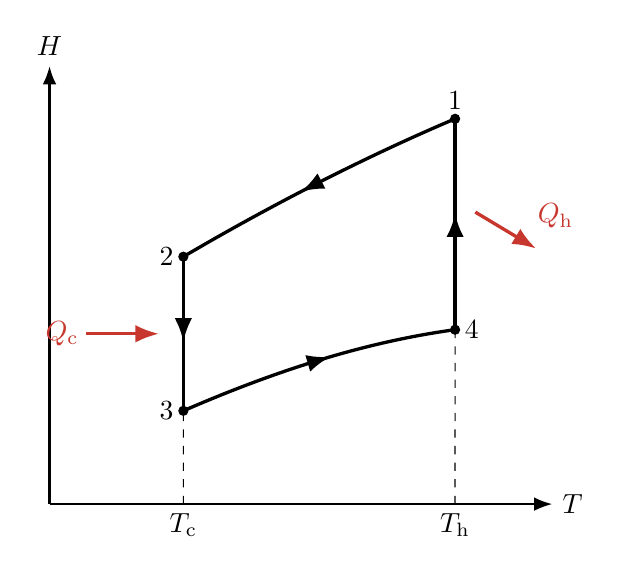
\begin{tikzpicture}[scale=1.03,>=Latex]
  \draw[->,thick] (0,0)--(6.2,0) node[right] {$T$};
  \draw[->,thick] (0,0)--(0,5.4) node[above] {$H$};
  \coordinate (p1) at (5.0,4.75);
  \coordinate (p2) at (1.65,3.05);
  \coordinate (p3) at (1.65,1.15);
  \coordinate (p4) at (5.0,2.15);
  \draw[very thick,postaction={decorate},decoration={markings,mark=at position .56 with {\arrow{Latex}}}] (p1) .. controls (3.7,4.2) and (2.5,3.55) .. (p2);
  \draw[very thick,postaction={decorate},decoration={markings,mark=at position .55 with {\arrow{Latex}}}] (p2)--(p3);
  \draw[very thick,postaction={decorate},decoration={markings,mark=at position .55 with {\arrow{Latex}}}] (p3) .. controls (2.8,1.65) and (3.9,2.0) .. (p4);
  \draw[very thick,postaction={decorate},decoration={markings,mark=at position .55 with {\arrow{Latex}}}] (p4)--(p1);
  \draw[dashed] (1.65,0)--(p2);
  \draw[dashed] (5.0,0)--(p1);
  \node[below] at (1.65,0) {$T_{\mathrm c}$};
  \node[below] at (5.0,0) {$T_{\mathrm h}$};
  \foreach \p/\lab/\pos in {p1/1/above,p2/2/left,p3/3/left,p4/4/right}{\fill (\p) circle (1.8pt) node[\pos] {$\lab$};}
  \draw[heatred,very thick,-{Latex[length=3mm]}] (0.45,2.1)--(1.35,2.1);
  \node[heatred,left] at (0.48,2.1) {$Q_{\mathrm c}$};
  \draw[heatred,very thick,-{Latex[length=3mm]}] (5.25,3.6)--(6.0,3.15);
  \node[heatred,right] at (5.9,3.55) {$Q_{\mathrm h}$};
\end{tikzpicture}

图 3b：顺磁卡诺制冷循环的 $H$--$T$ 图
\end{center}

\begin{solutionbox}
\textbf{T3-C1}

循环如图 3b 所示。低温等温段 $2\to3$ 吸收热量 $Q_{\mathrm c}$；高温等温段 $4\to1$ 向高温热库排出热量 $Q_{\mathrm h}$。两条弯曲轨迹 $1\to2$ 与 $3\to4$ 为绝热过程。

\textbf{T3-C2}

对可逆卡诺循环，
\[
\frac{Q_{\mathrm c}}{Q_{\mathrm h}}=\frac{T_{\mathrm c}}{T_{\mathrm h}}.
\]
由 T3-B1 的等温吸热公式，低温等温过程 $2\to3$ 中
\[
Q_{\mathrm c}
=-\frac{\mu_0nK}{2T_{\mathrm c}}(H_3^2-H_2^2)
=\frac{\mu_0nK}{2T_{\mathrm c}}(H_2^2-H_3^2).
\]
高温等温过程 $4\to1$ 中，系统吸收的热量为负，因此向热库排出的热量大小为
\[
Q_{\mathrm h}
=\frac{\mu_0nK}{2T_{\mathrm h}}(H_1^2-H_4^2).
\]
代入卡诺关系：
\[
\frac{T_{\mathrm h}}{T_{\mathrm c}}
\frac{H_2^2-H_3^2}{H_1^2-H_4^2}
=\frac{T_{\mathrm c}}{T_{\mathrm h}}.
\]
所以
\[
\frac{H_2^2-H_3^2}{T_{\mathrm c}^2}
=\frac{H_1^2-H_4^2}{T_{\mathrm h}^2}.
\]
由状态方程
\[
M=\frac{nKH}{TV},
\]
上式等价于
\[
M_2^2-M_3^2=M_1^2-M_4^2.
\]
于是
\begin{answerbox}
\[
\boxed{M_1=\sqrt{M_2^2-M_3^2+M_4^2}}.
\]
\end{answerbox}

\textbf{T3-C3}

低温端每循环吸收的热量为
\[
Q_{\mathrm c}=\frac{\mu_0nK}{2T_{\mathrm c}}(H_2^2-H_3^2).
\]
代入数值：
\begin{align*}
Q_{\mathrm c}
&=\frac{(4\pi\times10^{-7})(1.00\times10^{-2})(2.74\times10^{-5})}{2(1.00)}\\
&\quad\times\left[(1.00\times10^6)^2-(5.00\times10^5)^2\right]\\
&=1.29\times10^{-1}\ \mathrm J.
\end{align*}
液氦质量为
\[
m_{\rm He}=\rho_{\rm He}V_{\rm He}
=130\times10^{-3}=0.130\ \mathrm{kg}.
\]
其温降大小为
\[
|\Delta T|_{\rm He}
=\frac{Q_{\mathrm c}}{m_{\rm He}c_{\rm He}}
=\frac{1.29\times10^{-1}}{0.130\times10^2}
=9.92\times10^{-3}\ \mathrm K.
\]
因此
\begin{answerbox}
\[
\boxed{Q_{\mathrm c}=1.29\times10^{-1}\ \mathrm J},
\qquad
\boxed{T_f=1.00-0.00992=0.99008\ \mathrm K}.
\]
\end{answerbox}

\textbf{T3-C4}

在某一瞬间，冷端温度为 $T_{\mathrm c}$。对微小卡诺制冷循环，
\[
\frac{\dd Q_{\mathrm c}}{\dd Q_{\mathrm h}}=\frac{T_{\mathrm c}}{T_{\mathrm h}}.
\]
第一定律给出
\[
\dd Q_{\mathrm h}=\dd W+\dd Q_{\mathrm c}.
\]
恒定输入功率意味着
\[
\dd W=P\dd t.
\]
冷端物体温度下降 $\dd T_{\mathrm c}<0$ 时，制冷机吸收
\[
\dd Q_{\mathrm c}=-C_{\mathrm c}\dd T_{\mathrm c}.
\]
因此
\[
\frac{\dd W+\dd Q_{\mathrm c}}{\dd Q_{\mathrm c}}
=\frac{T_{\mathrm h}}{T_{\mathrm c}},
\]
即
\[
-\frac{P\dd t}{C_{\mathrm c}\dd T_{\mathrm c}}+1
=\frac{T_{\mathrm h}}{T_{\mathrm c}}.
\]
整理为
\[
\dd t=-\frac{C_{\mathrm c}T_{\mathrm h}}{P}
\left(\frac{\dd T_{\mathrm c}}{T_{\mathrm c}}
-\frac{\dd T_{\mathrm c}}{T_{\mathrm h}}\right).
\]
从 $t=0,T_{\mathrm c}=T_0$ 积分到 $t,T_{\mathrm c}=T$：
\begin{align*}
t
&=-\frac{C_{\mathrm c}T_{\mathrm h}}{P}
\int_{T_0}^{T}\left(\frac1{T_{\mathrm c}}-\frac1{T_{\mathrm h}}\right)\dd T_{\mathrm c}\\
&=\frac{C_{\mathrm c}T_{\mathrm h}}{P}
\left[\ln\frac{T_0}{T}-\frac{T_0-T}{T_{\mathrm h}}\right].
\end{align*}
故
\begin{answerbox}
\[
\boxed{t=\frac{C_{\mathrm c}T_{\mathrm h}}{P}
\left(\ln\dfrac{T_0}{T}-\dfrac{T_0-T}{T_{\mathrm h}}\right)}.
\]
\end{answerbox}
当 $T\to0$ 时，$\ln(T_0/T)\to\infty$，因此达到绝对零度需要无限长时间。

\textbf{T3-C5}

整个过程中从冷端吸收的总热量为
\[
Q_{\mathrm c}=C_{\mathrm c}(T_0-T).
\]
总输入功为
\[
W=Pt
=C_{\mathrm c}T_{\mathrm h}\ln\frac{T_0}{T}
-C_{\mathrm c}(T_0-T)
=C_{\mathrm c}T_{\mathrm h}\ln\frac{T_0}{T}-Q_{\mathrm c}.
\]
因此平均性能系数为
\begin{align*}
\mathrm{COP}
&=\frac{Q_{\mathrm c}}{W}\\
&=\frac{C_{\mathrm c}(T_0-T)}{C_{\mathrm c}T_{\mathrm h}\ln(T_0/T)-C_{\mathrm c}(T_0-T)}.
\end{align*}
化简得到
\begin{answerbox}
\[
\boxed{\mathrm{COP}
=\left[\frac{T_{\mathrm h}}{T_0-T}\ln\frac{T_0}{T}-1\right]^{-1}}.
\]
\end{answerbox}
当目标温度 $T$ 越接近零，平均性能系数越趋近于零，制冷效率急剧下降。
\end{solutionbox}

\section*{答案汇总}
\begin{answerbox}
\begin{align*}
\text{T3-A1:}\quad &H=\frac{NIA}{V},\\
\text{T3-A2:}\quad &\dd W_{\rm emf}=VH\,\dd B,\\
\text{T3-A3:}\quad &\dd W=\mu_0VH\,\dd M,\\[0.3em]
\text{T3-B1:}\quad &Q=-\frac{\mu_0nK}{2T}(H_f^2-H_i^2),\\
\text{T3-B2:}\quad &\Delta T=T_i\left[\sqrt{\frac{\lambda+\mu_0KH_f^2}{\lambda+\mu_0KH_i^2}}-1\right],\\[0.3em]
\text{T3-C2:}\quad &M_1=\sqrt{M_2^2-M_3^2+M_4^2},\\
\text{T3-C3:}\quad &Q_{\mathrm c}=1.29\times10^{-1}\ \mathrm J,\qquad T_f=0.99008\ \mathrm K,\\
\text{T3-C4:}\quad &t=\frac{C_{\mathrm c}T_{\mathrm h}}{P}
\left(\ln\frac{T_0}{T}-\frac{T_0-T}{T_{\mathrm h}}\right),\\
\text{T3-C5:}\quad &\mathrm{COP}=\left[\frac{T_{\mathrm h}}{T_0-T}\ln\frac{T_0}{T}-1\right]^{-1}.
\end{align*}
\end{answerbox}

\end{document}
